\documentclass[11pt]{article}
\usepackage{fontspec}\setmainfont{Times New Roman}
\usepackage[paperwidth=595.32bp,paperheight=841.92bp,left=80bp,right=80bp,top=111bp,bottom=104bp]{geometry}
\usepackage{amsmath,amssymb,booktabs,longtable,array,pdfpages,hyperref,eso-pic,graphicx}
\hypersetup{hidelinks,pdftitle={BSE3124 Group 1 Final Answer Sheets}}
\pagestyle{empty}\setlength{\parindent}{0pt}\setlength{\parskip}{5pt}
\setlength{\tabcolsep}{4pt}\renewcommand{\arraystretch}{1.16}\emergencystretch=2em
\setlength{\unitlength}{1bp}
\newcommand{\slot}[4]{\put(#1,\dimexpr841.92bp-#2bp\relax){\makebox(0,0)[lt]{\begin{minipage}[t]{#3bp}\vspace{0pt}\fontsize{11}{13}\selectfont\setlength{\parskip}{5pt} #4\end{minipage}}}}
% Match the teacher's restrained heading hierarchy.
\makeatletter
\renewcommand\section{\@startsection{section}{1}{0pt}{12pt}{7pt}{\normalfont\fontsize{12}{14}\selectfont\bfseries}}
\renewcommand\subsection{\@startsection{subsection}{2}{0pt}{10pt}{5pt}{\normalfont\fontsize{11}{13}\selectfont\bfseries}}
\makeatother
\newcommand{\tenantselection}{\textbf{The office tenant chosen for layout design: Office 1.}}
\newcommand{\task}[1]{\section*{#1}}
\widowpenalty=10000\clubpenalty=10000
\AddToShipoutPictureFG{\ifnum\value{page}>1\AtPageLowerLeft{\put(\dimexpr0.5\paperwidth\relax,24){\makebox(0,0){\fontsize{9}{11}\selectfont\thepage}}}\fi}
\newcommand{\sheet}[2]{\long\gdef\currentsheetoverlay{#2}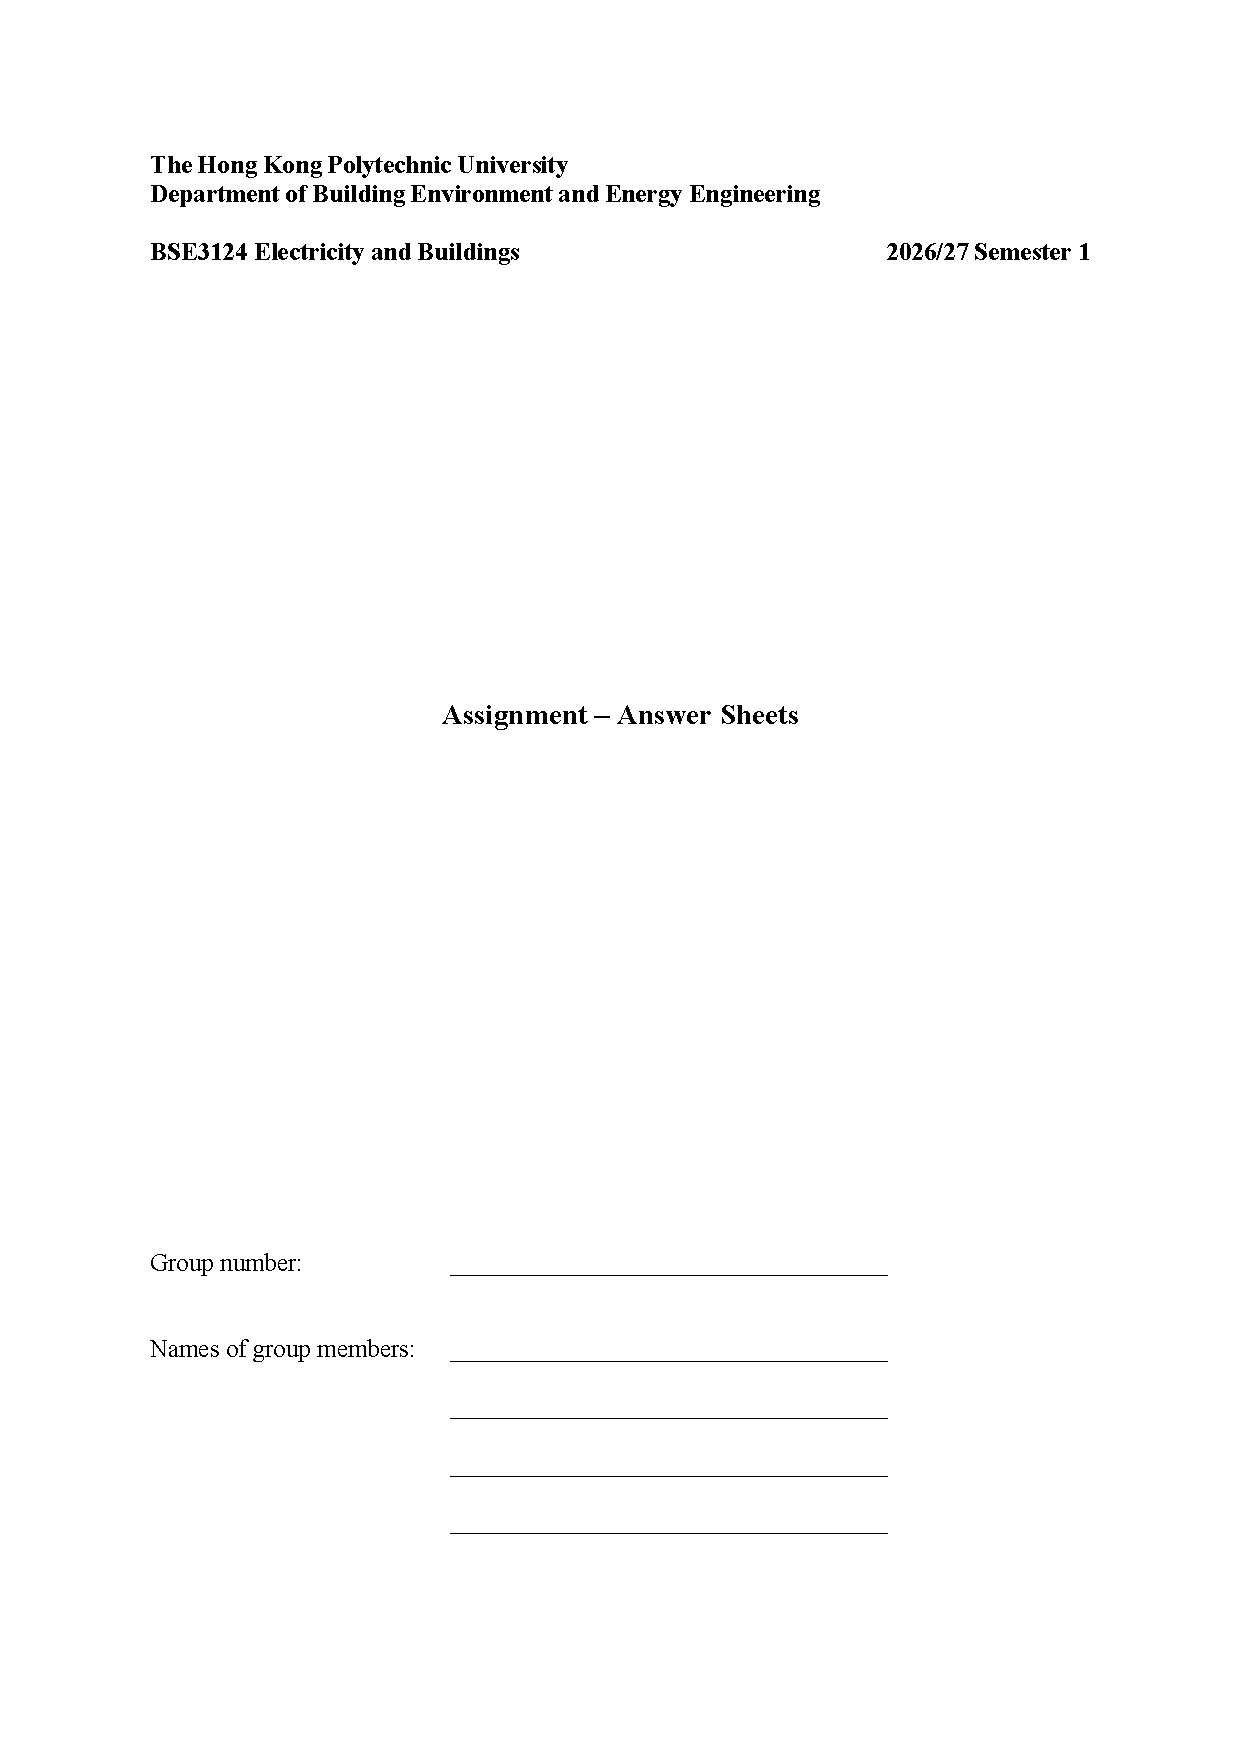
\includepdf[pages=#1,fitpaper=true,noautoscale=true,pagecommand={\AddToShipoutPictureFG*{\AtPageLowerLeft{\currentsheetoverlay}}}]{assets/official-template.pdf}}
\begin{document}
\sheet{1}{
\slot{220}{599}{205}{1}
\slot{220}{640}{205}{LYU Mingliang (24099296D)}
\slot{220}{668}{205}{HUANG Celine (24034414D)}
\slot{220}{696}{205}{LIU Wing Kei (24093229D)}}
\sheet{2}{\slot{80}{153}{435}{
\textbf{Basis and assumptions.} The assessment covers ten identical office floors, each with usable areas assumed to be 309, 309 and 410\,m$^2$. CLP COP215 Rev 07 forms the load-assessment basis. The 1000\,kW in the question is cooling output, not electrical demand. Additionally, the calculation assumes packaged air-cooled AC, PF 0.90, five lifts and equal allocation to two supply zones.
\begin{align*}
A&=10(309+309+410)=10\,280\ {\rm m^2},\\
S_{\rm office}&=10\,280(0.16)=1644.8\ {\rm kVA},\\
P_{\rm AC}&=(1000/3.51685)(1.85)=526.039\ {\rm kW},\\
S_{\rm AC}&=526.039/0.90=584.488\ {\rm kVA},\\
S_{\rm public}&=5(40)=200\ {\rm kVA},\\
S_{\rm design}&=1.10(1644.8+584.488+200)=2672.216\ {\rm kVA}.
\end{align*}
The 40\,kVA/lift allowance is an aggregate public-services reference, not a lift motor rating. A public-services overlap allowance of 0--200\,kVA gives 2452.216--2672.216\,kVA; the upper bound is adopted. The references are COP215 3.1.7, 3.3.1 and Appendices 2/7.

\textbf{Selection.} The proposal uses two 1500\,kVA transformers to provide 3000\,kVA. Each serves five floors and half the plant/public allowance: 1336.108\,kVA per section. Full-load N--1 is not provided; a failed transformer requires load shedding. Unauthorised parallel operation must be prevented.

\textbf{Room location.} The lower-left ground-floor perimeter accommodates the proposed 12430$\times$5450\,mm transformer room and adjacent 12430$\times$3500\,mm main LV room (LV depth assumed). This allows external delivery/access, short LV interfaces, separation from the central lift/stair/AHU core and independent customer access.

Access provisions include 3\,m delivery access within 20\,m of unloading. Its planning conditions include COP101 v16 4.3 clearance envelopes, 2-hour partitions, sealed penetrations and a raised floor level. Door sweeps require sequential use. Louvres provide 1.20\,m$^2$ free area at the assumed 50\% free ratio. Equipment/ventilation and 10.03/10.31\,m LV interfaces are detailed in the continuation and ground-floor drawings.
}}
\AddToShipoutPictureBG{\AtPageLowerLeft{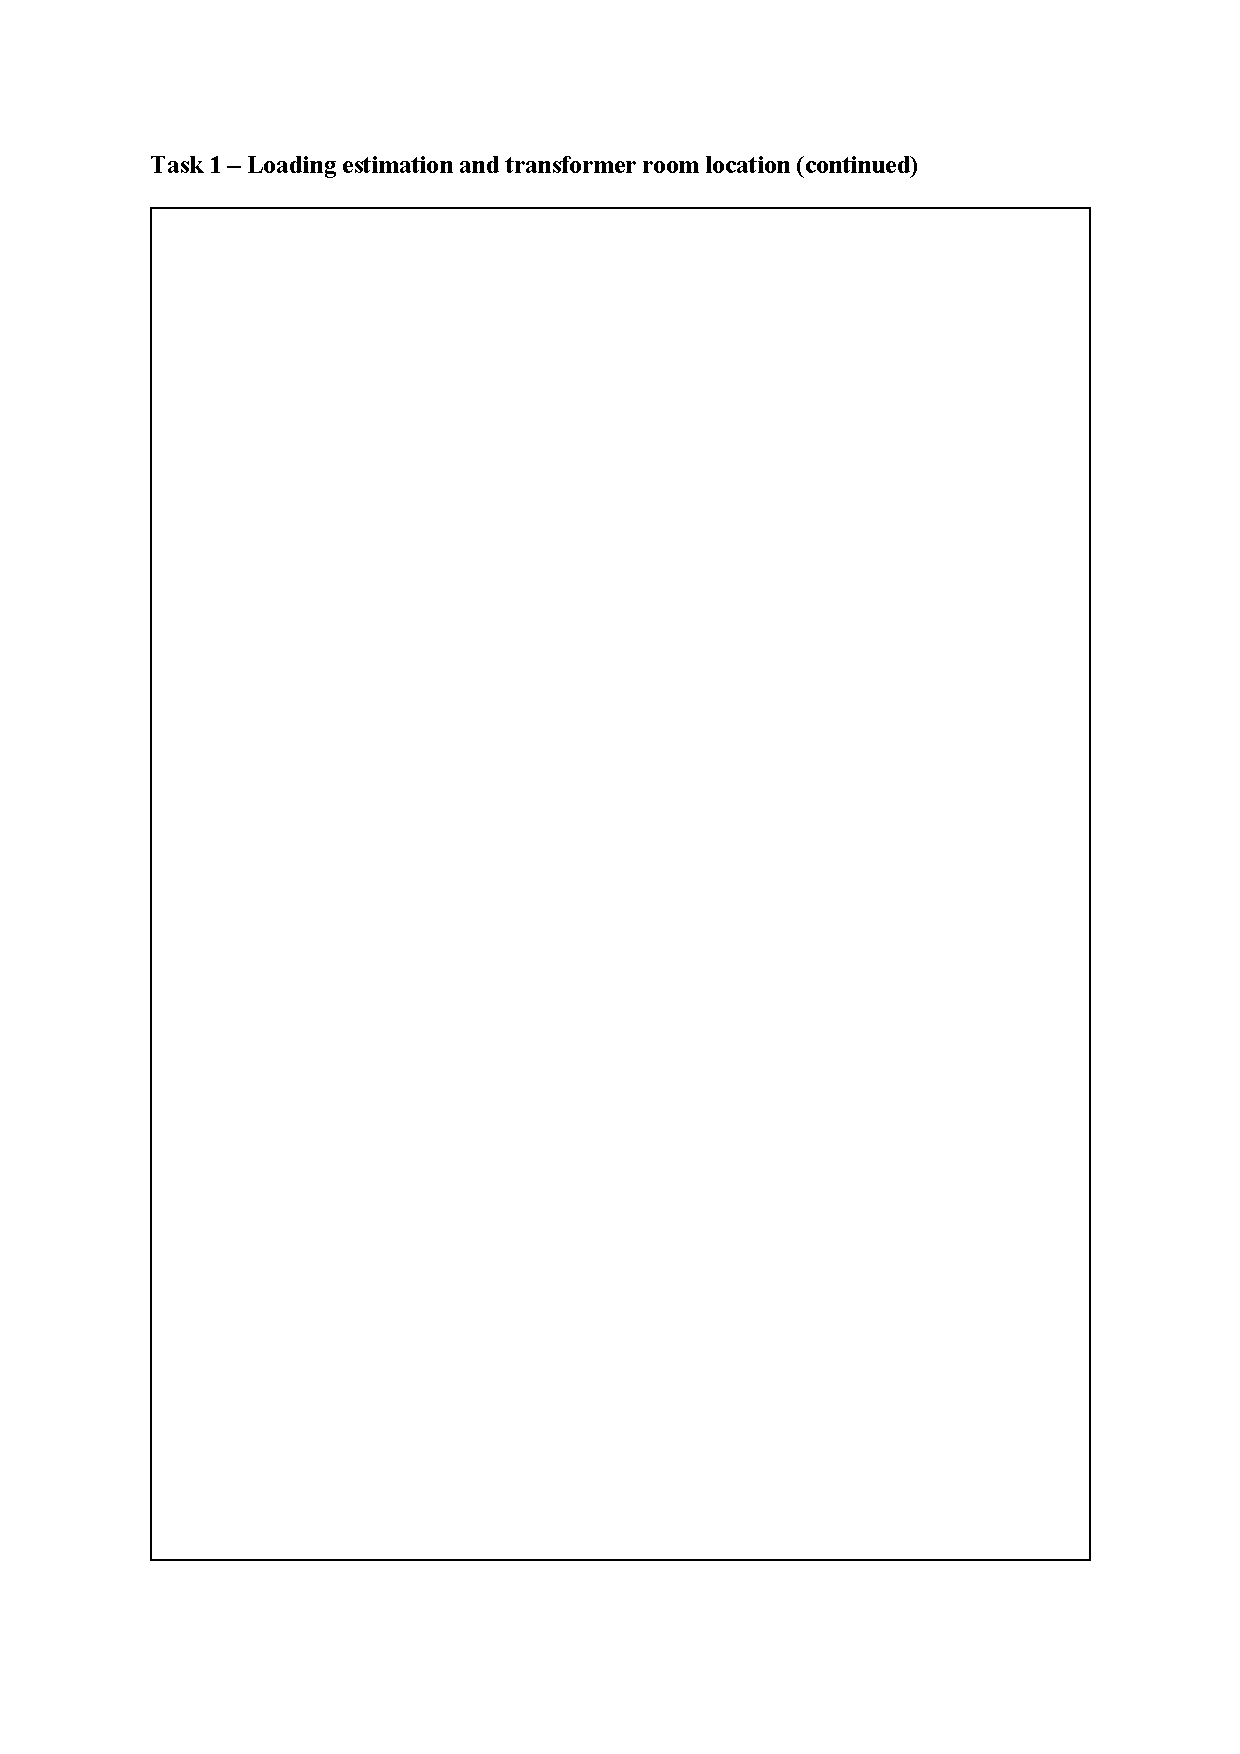
\includegraphics[page=1,width=\paperwidth,height=\paperheight]{assets/continuation-template.pdf}}}
% !TeX root = main.tex
\subsection*{Transformer and main LV room proposal}
The proposal starts with two 1500 kVA transformers serving separate LV sections, providing 3000 kVA in total and a margin of 327.784 kVA. Floors 1--5 are allocated to section A and floors 6--10 to section B, with each section also receiving half of the central plant/public allowance. Under this assumed equal split, each section carries 1336.108 kVA, corresponding to about 2030 A at 380 V. However, full-load N--1 is not provided, so load shedding is required if one unit is lost. The two LV sections operate independently; no bus coupler is provided.

Room placement follows the lower-left perimeter of the supplied plan, with a 12430 by 5450 mm substation and an adjacent 12430 by 3500 mm LV room, whose depth is assumed. This location allows external plant access and short LV interfaces, while providing separation from the lift/stair/AHU core and independent LV access. Additionally, a 3 m clear delivery route within 20 m of unloading is proposed, subject to confirmation of the external site conditions.

The plantroom drawing shows HV-01 as a compartmented switchboard and TX-A/TX-B as transformer plan symbols with HV/LV terminal positions. Adopted overall dimensions are 3000 by 1000 mm for HV-01 and 2200 by 1800 mm for each transformer, with six LV cabinets. These are design dimensions; internal equipment details are diagrammatic. Their clearance envelopes fit without overlap. COP101 v 16 clause 4.3 requires HV clearances of 1000 mm at the rear, 1800 mm at the front and 750 mm at the sides, together with 900 mm at transformer LV terminals and 750 mm elsewhere. Additionally, the proposal includes 2-hour partitions, sealed penetrations and an FFL 150 mm above external level. Meanwhile, the outward-opening 180-degree doors have shared sweeps and therefore require sequential use.

Ventilation is provided by two 600 by 2000 mm louvres, providing 1.20 m$^2$ at an assumed 50\% free-area ratio, above clause 6.3's 1.12 m$^2$ reference. Thus, the certified free-area ratio must be at least 46.67\%. Fan symbols are conditional provisions, not actual heat-loss calculations. Meanwhile, the LV interfaces, including the assumed tails, are 10.03/10.31 m, below the 20 m limit in 5.5.2.2. Actual equipment, structures, openings and ventilation must satisfy these declared conditions.

\subsection*{Main distribution schematic}
The main schematic connects TX-A and TX-B through their respective ACB incomers to MSB-A and MSB-B. Separate rising supplies serve floors 1--5 and 6--10, with three tenants per floor. Each section also feeds its allocated central plant and public services. The Office 1 inset links floor metering to MS-O1, the selected feeder and DB-O1. The arrangement follows the transformer, switchboard and metering relationships in \emph{Electrical Schematic 1}; the adopted loads and final-circuit ratings remain those calculated in Tasks 1 and 3.

\clearpage\ClearShipoutPictureBG
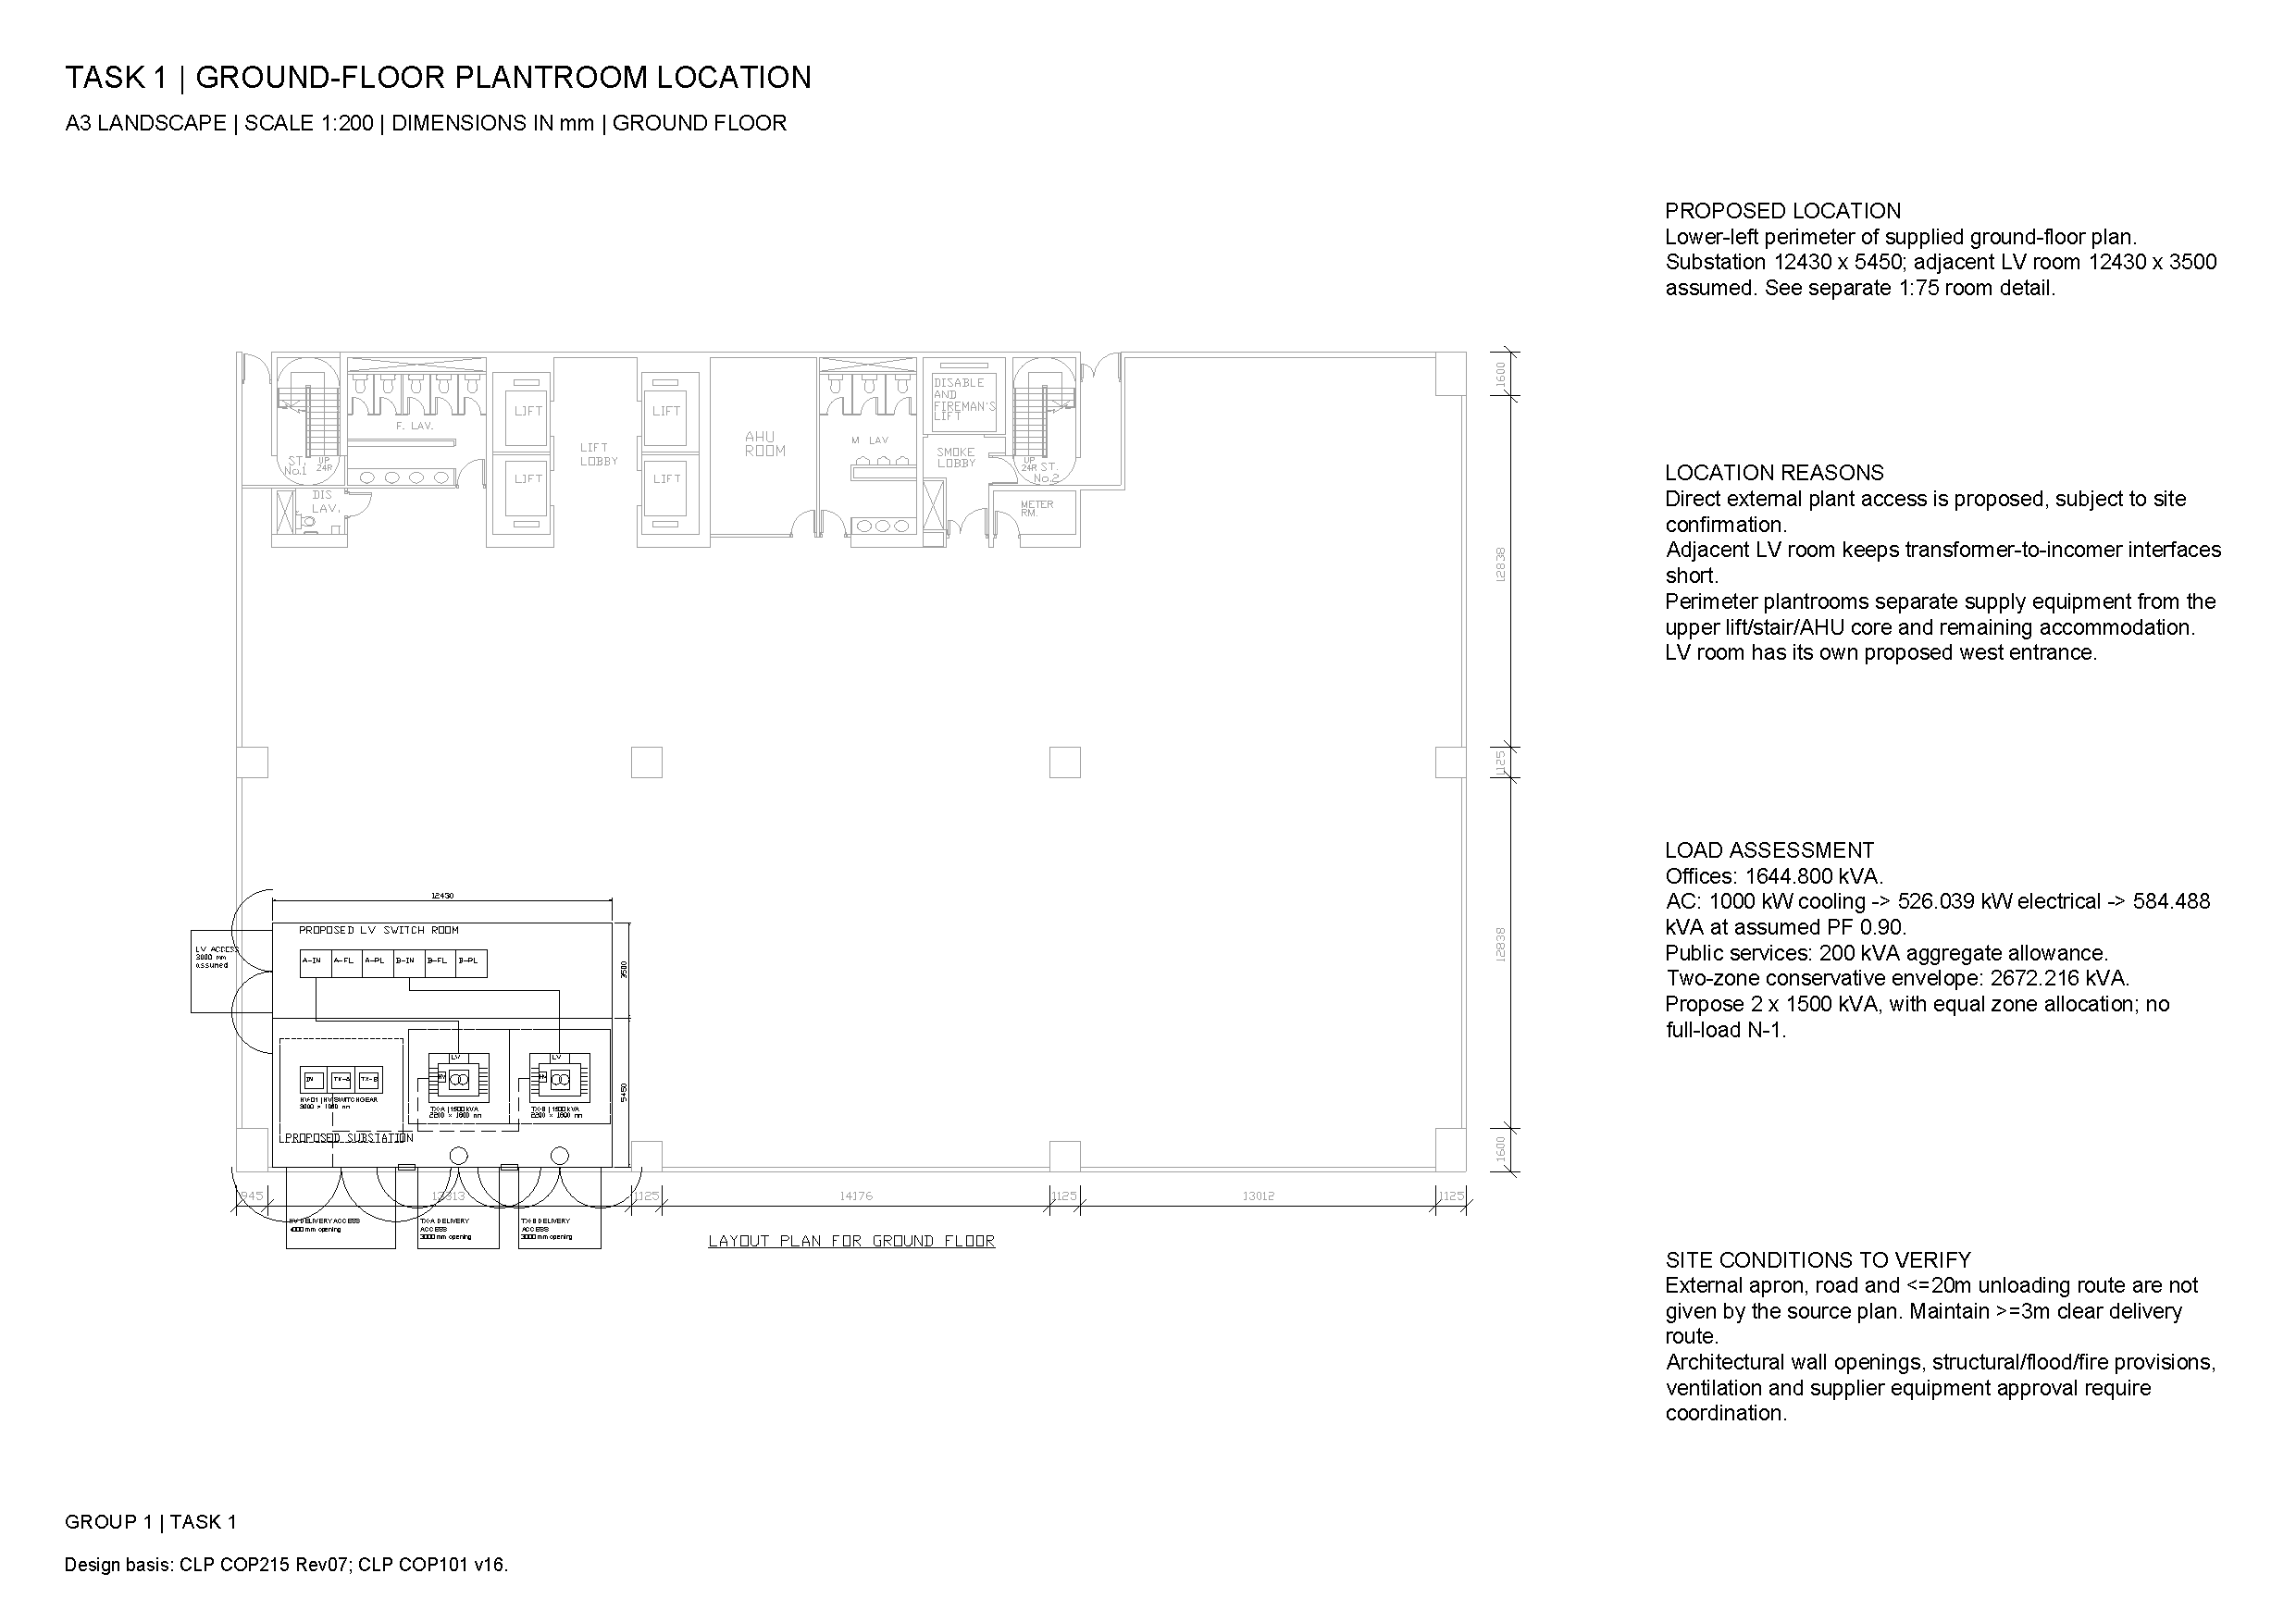
\includepdf[pages=-,fitpaper=true]{assets/task1-drawings.pdf}
\sheet{3}{
% Replace the unselected template options with the adopted tenant.
\put(76,711){\color{white}\rule{445bp}{18bp}}
\slot{77.664}{114}{435}{\fontsize{12}{14}\selectfont\tenantselection}
\slot{80}{181}{435}{
\textbf{Selected tenant: Office 1.} The attached lighting/power plans, completed board template and detailed L/N/PE schematic present the design.

\textbf{Lighting.} Normal lighting uses 92 PIL PLATO 600 panels: sixty 22\,W, twenty-eight 28\,W and four 38\,W, total 2256\,W. Seven circuits LC-A--LC-G have 18/17/18/11/14/10/4 lamps, each protected by B10 Type A 30\,mA 1P+N RCBO. Each has its own neutral and local manual control S-A--S-G. Different-phase switches use separate enclosures. Ceiling-grid and furniture relationships guide positions.

\textbf{Lighting performance.} Manufacturer LDT calculations give maintained mean direct illuminances of 592.9/546.3/588.5/662.6\,lx for the open office/pantry/upper east/south east rooms at 1.9\,m above the workplane and MF 0.80. Four 38\,W panels in the south east room retain 589.2\,lx at 2.2\,m, providing a 17.8\% margin above the 500\,lx design target. The continuation gives the calculation method and room results.

\textbf{Power.} Small-power provision comprises nine four-socket floorboxes, three twin sockets and FS01. Every assembly has one upstream 13\,A FCU; its outlets share that capacity. P1--P4 use 6\,mm$^2$ A1 rings/B32, P5/P6/P8 use 10\,mm$^2$ A2 radials/B32, and P7 uses a 4\,mm$^2$ dedicated radial/B16. Each local fused spur is 4\,mm$^2$, assumed 0.5\,m. FCUs precede the spur cable. Additionally, the pantry circuits are separated from ordinary office circuits. FS01 reserves 13\,A without inventing an appliance rating.

\textbf{Protection and containment.} Ring protection requires L/N/CPC continuity, with both ends returning to the same circuit under EMSD Table 6(1)'s A1 ring conditions. The lighting group, ring banks A/B, radial bank C, P7 and incoming feeder remain separate to preserve the stated grouping factors, as shown on the installation-detail sheet.

\textbf{Supply and controls.} The supply uses source C63 4P protection, 4C35\,mm$^2$ + CPC16 and 100\,A 4P DB isolation. Dedicated neutrals pass through their own RCBO; PE is unswitched. Accordingly, the selected apparatus must meet the specified 10\,kA breaking capacity and total-energy/inrush limits. Landlord emergency lighting and exit signs use independent essential supplies.
}}
\AddToShipoutPictureBG{\AtPageLowerLeft{\includegraphics[page=2,width=\paperwidth,height=\paperheight]{assets/continuation-template.pdf}}}
% !TeX root = main.tex
{\fontsize{12}{14}\selectfont\tenantselection}
\subsection*{Normal lighting and local controls}
The lighting proposal starts with 92 PIL PLATO 600 MultiPower 3117955 panels on the 600 mm ceiling grid: sixty 22 W, twenty-eight 28 W and four 38 W, totalling 2256 W. Their nominal fluxes are 2843.45, 3555.30 and 4685.55 lm respectively. Separate circuits serve the enclosed rooms and distributed main-office zones, with a maintained mean illuminance target of 500 lx adopted for the design. With this arrangement, the connected lighting density is 7.301 W/m$^2$ using the adopted 309 m$^2$ office area.

Seven passive manual switches S-A--S-G provide local control of their corresponding circuits. These switches must have a minimum rating of 20 AX, an LED switching capacity of at least 600 W and make/break/inrush compatibility with the selected drivers. Since their phases differ, S-A/B/C use separate enclosures. No borrowed neutral is allowed. Each route passes through its switch and includes a 2 m DB rise plus 1.5 m down and 1.5 m back at the switch, giving an assumed vertical allowance of 5 m per lighting radial. Passive controls add no operating power.
\begin{center}\begin{tabular}{lrrrrl}\toprule
Circuit & Lamps & W & Phase & RCBO & Control\\\midrule

LC-A & 18 & 402 & L1 & B10 & S-A \\
LC-B & 17 & 392 & L2 & B10 & S-B \\
LC-C & 18 & 396 & L3 & B10 & S-C \\
LC-D & 11 & 242 & L3 & B10 & S-D \\
LC-E & 14 & 392 & L2 & B10 & S-E \\
LC-F & 10 & 280 & L1 & B10 & S-F \\
LC-G & 4 & 152 & L3 & B10 & S-G \\

\bottomrule\end{tabular}\end{center}
On the plan, the A/B/C numeric labels correspond to the LED IDs and circuits LC-A/B/C. Similarly, D01--D11 correspond to PN01--PN11, E82--E96 excluding E90 to the northeast LEDs, F01--F10 to UE01--UE10, and G01--G04 to SE01--SE04. Power settings follow the common device schedule. Every luminaire and control has one circuit assignment.
% !TeX root = main.tex
\subsection*{Lighting calculation}
To assess lighting performance, the calculation uses manufacturer LDT intensities given in cd/klm, with each profile scaled by its selected flux: 2843.45 lm at 22 W, 3555.30 lm at 28 W and 4685.55 lm at 38 W. Illuminance is then calculated at each workplane grid cell, with spacing at most 0.2 m, as
\[
E=0.80\sum_j\frac{I_j(C,\gamma)\cos\gamma}{d_j^2}.
\]
A luminaire-to-workplane height of 1.9 m is adopted, corresponding to a 2.7 m ceiling and a 0.8 m workplane. Meanwhile, the maintenance factor of 0.80 assumes periodic cleaning and replacement. Room boundaries use the adopted plan envelopes; each room receives light from its own fittings. Only direct light is included in this calculation.
\begin{center}\begin{tabular}{lrrrr}\toprule
Zone & Lamps & Area m$^2$ & Mean lx & Min/mean\\\midrule
Open office & 67 & 231.87 & 592.9 & 0.136\\
Pantry & 11 & 29.54 & 546.3 & 0.390\\
Upper east room & 10 & 33.68 & 588.5 & 0.267\\
South east room & 4 & 13.07 & 662.6 & 0.175\\
\bottomrule\end{tabular}\end{center}
On this basis, all four mean illuminances exceed the adopted 500 lx target. To provide mounting-height tolerance, the four south-east panels use the 38 W setting. At 2.2 m above the workplane, the respective means are 573.0, 505.8, 545.0 and 589.2 lx; the south-east room retains a 17.8\% margin.

When interpreting these results, the minimum/mean ratios include perimeter cells. Overall, the assessment covers mean direct illuminance; a detailed task-area check would also account for furniture, reflections and glare.

\subsection*{Small power and fixed equipment}
Small-power provision includes nine four-socket floor boxes, three twin wall sockets and the fixed connection FS01. Each floor-box/socket assembly is individually 13 A fused. Accordingly, the demand calculation uses a 13 A continuous capacity per assembly; FS01 reserves a further 13 A for fixed equipment. Meanwhile, building central AC is supplied as central plant and not duplicated in this office DB.

P1--P4 are A1 rings with fused floor-box connections. In comparison, P5/P6/P8 are A2 radials, while P7 is a fixed radial. Both P6 and P8 serve the PANTRY identified on the source plan, with FB09 and SO01 connected to P6. P8 is a separate socket group for convenient isolation. Kitchen sockets are separated from ordinary office circuits under EMSD6E(3)(a).
\begin{center}\begin{tabular}{llllr}\toprule
Circuit & Points & Phase & Topology & Protection\\\midrule

P1 & FB01, FB02 & L1 & A1 ring & B32 \\
P2 & FB03, FB04 & L1 & A1 ring & B32 \\
P3 & FB05, FB06 & L2 & A1 ring & B32 \\
P4 & FB07, FB08 & L2 & A1 ring & B32 \\
P5 & SO02 & L1 & A2 radial & B32 \\
P6 & FB09, SO01 & L3 & A2 radial & B32 \\
P7 & FS01 & L3 & Fixed radial & B16 \\
P8 & SO03 & L3 & A2 radial & B32 \\

\bottomrule\end{tabular}\end{center}
In terms of coverage, the defined service envelopes satisfy the A1 maximum of 100 m$^2$ and the A2 maximum of 50 m$^2$. Coverage is assessed by service envelope, allowing overlap between circuits. Ring L/N/CPC return to their own circuit terminals. Main 6/10 mm$^2$ cables terminate in accessible junction/FCU assemblies rated for those conductor sizes. At each point, the local connections use 4 mm$^2$ L/N/CPC, with an assumed length of 0.5 m per point.
\clearpage
% !TeX root = main.tex
\subsection*{FCU and containment details}
Every FB01--FB09 assembly shares one 13 A FCU upstream of all four socket ways. Each twin SO01--SO03 likewise shares one 13 A FCU; FS01 has its own switched 13 A FCU. Ring/main L/N/CPC connections must terminate in an accessible junction assembly rated for 6/10 mm$^2$ cables. At each connection, the FCU is positioned at the tap before the 4 mm$^2$ local spur, with its neutral switched together with the line and its PE kept continuous. With 13 A continuous capacity per assembly as the demand basis, any added points require recalculation.

To maintain the adopted grouping factors, the containment is arranged in the following banks: lighting LC-A--G (seven circuits, $C_g=0.54$); A: P1/P2 (four ring legs, 0.65); B: P3/P4 (four ring legs, 0.65); C: P5/P6/P8 (three radials, 0.70); P7 alone (1.00); incoming feeder alone (1.00). Co-located plan paths show routing corridors, not a shared enclosure. Accordingly, separate Method B runs must provide horizontal clear space between groups exceeding twice the largest adjacent overall cable diameter, in accordance with EMSD A5(3), Note 2; where enclosure dimensions govern, the enclosures must be spaced at least as conservatively and the cable separation must be confirmed. Thermal separation is provided by cable clearance, rather than a partition alone. Within each circuit, L/N/CPC stays together. Additionally, contact with thermal insulation must be avoided. If these conditions cannot be achieved, the circuits must be regrouped and resized before installation.

\subsection*{Protection and board arrangement}
As shown in the complete schematic, the arrangement includes C63 four-pole protection at MS-O1, 4-core 35 mm$^2$ plus CPC16, a 100 A four-pole DB isolator, independent L1/L2/L3/N/PE bars and 15 separate 1P+N Type A 30 mA RCBOs. Every load neutral passes through its own RCBO;  none are shared downstream. Meanwhile, PE bypasses all switches. Additionally, the circuits and phases are to be labelled, and the arrangement must allow each final circuit to be isolated without interrupting the others.

Device selection must ensure that the proposed B-curve final protection is compatible with driver inrush and the breaking-capacity/energy limits established in Task 3. Individual RCBOs limit the effect of a residual-current fault to its own circuit; however, full short-circuit selectivity requires manufacturer coordination data.
\subsection*{Emergency lighting assumption}
Landlord emergency lighting and exit signage use independent essential supplies, separated from normal lighting under EMSD 6B(4). These feeds bypass tenant normal-lighting switches and RCBO load sides. Emergency-system loads are therefore outside this office normal-supply DB.

\clearpage\ClearShipoutPictureBG
\sheet{5}{\put(105,190){\rotatebox{90}{\begin{minipage}{450bp}\fontsize{9}{11}\selectfont\textbf{DB-O1: 8-way TPN chassis; 15 used single-phase outgoing positions}\par\smallskip\begin{tabular}{llll}\toprule Way & L1 & L2 & L3\\\midrule
1 & LC-A / B10 & LC-B / B10 & LC-C / B10\\
2 & LC-F / B10 & LC-E / B10 & LC-D / B10\\
3 & P1 / B32 & P3 / B32 & LC-G / B10\\
4 & P2 / B32 & P4 / B32 & P6 / B32\\
5 & P5 / B32 & Spare & P7 / B16\\
6 & Spare & Spare & P8 / B32\\
7 & Spare & Spare & Spare\\
8 & Spare & Spare & Spare\\
\bottomrule\end{tabular}\par\smallskip
Positions indicate phase allocation; each RCBO also needs its own N path. Additionally, the chassis/module capacity for 1P+N devices must be confirmed. The incoming protection is C63 4P at MS-O1, while the local main switch is 100A 4P (including N), supplementing the template's TP SW symbol. The detailed appended schematic governs neutral/PE connections and ring returns. All final RCBOs are Type A, 30mA, 10kA and must meet the energy/inrush specifications.\end{minipage}}}}
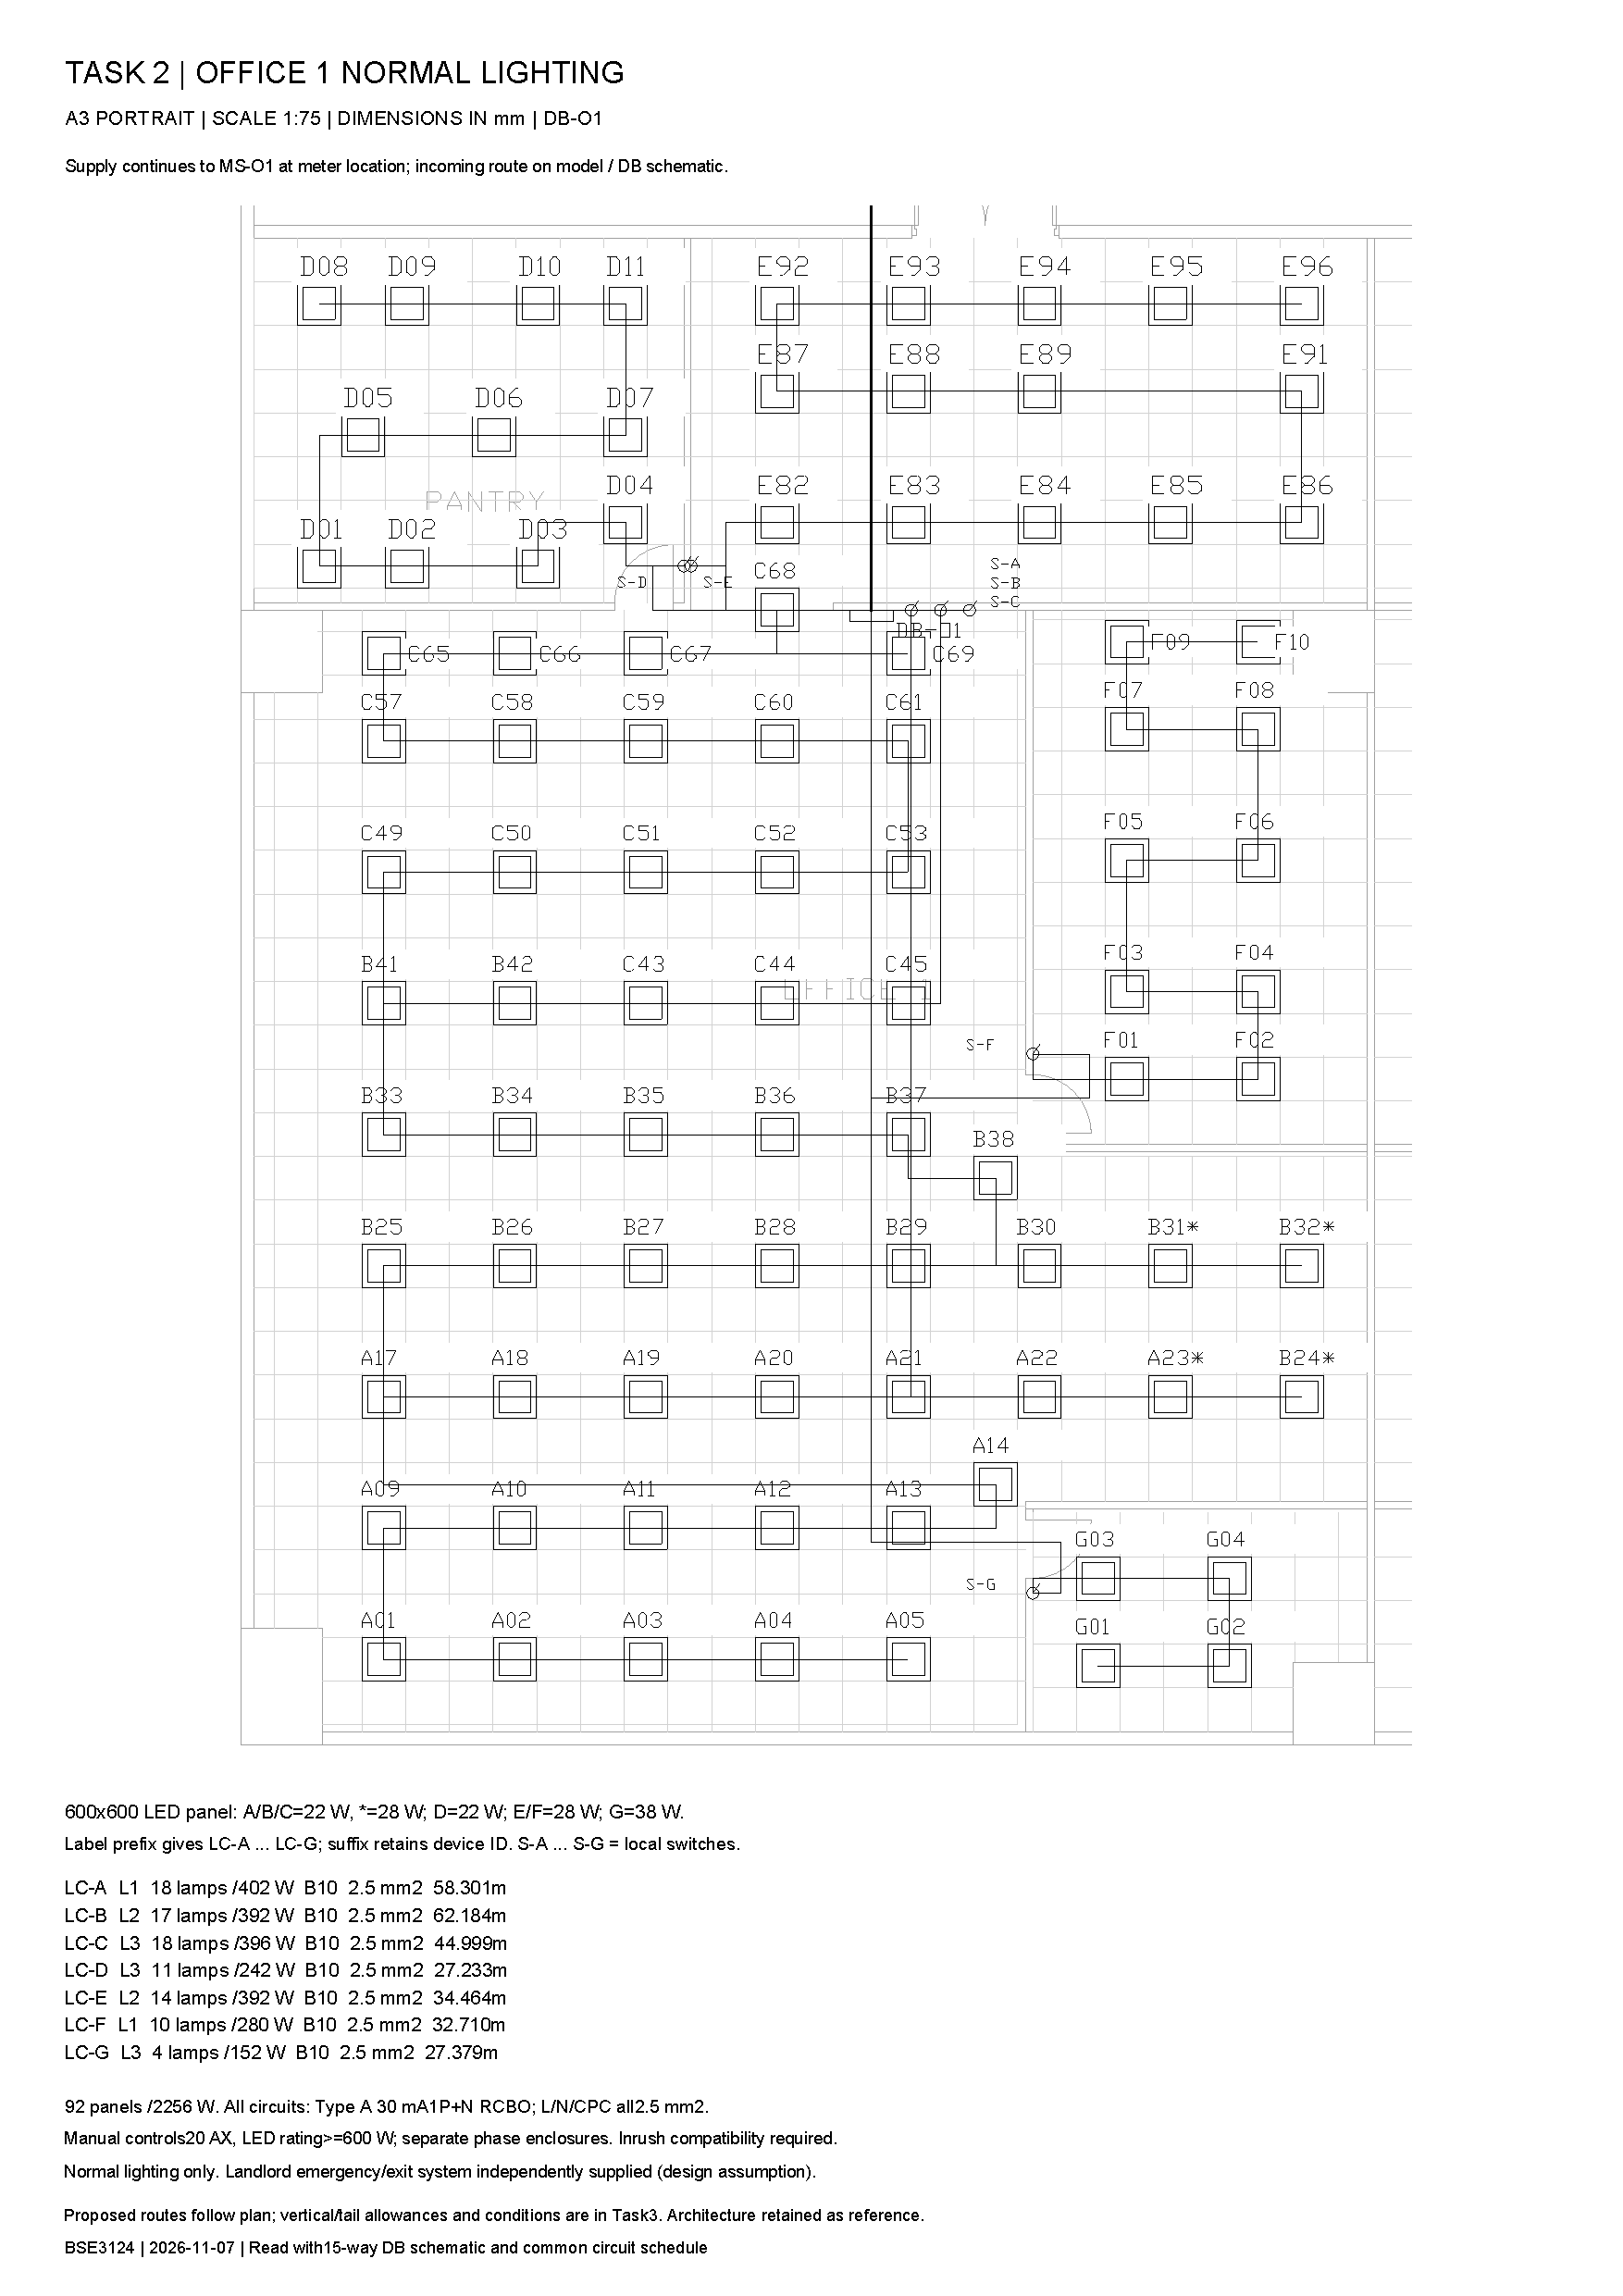
\includepdf[pages=-,fitpaper=true]{assets/office-lighting.pdf}
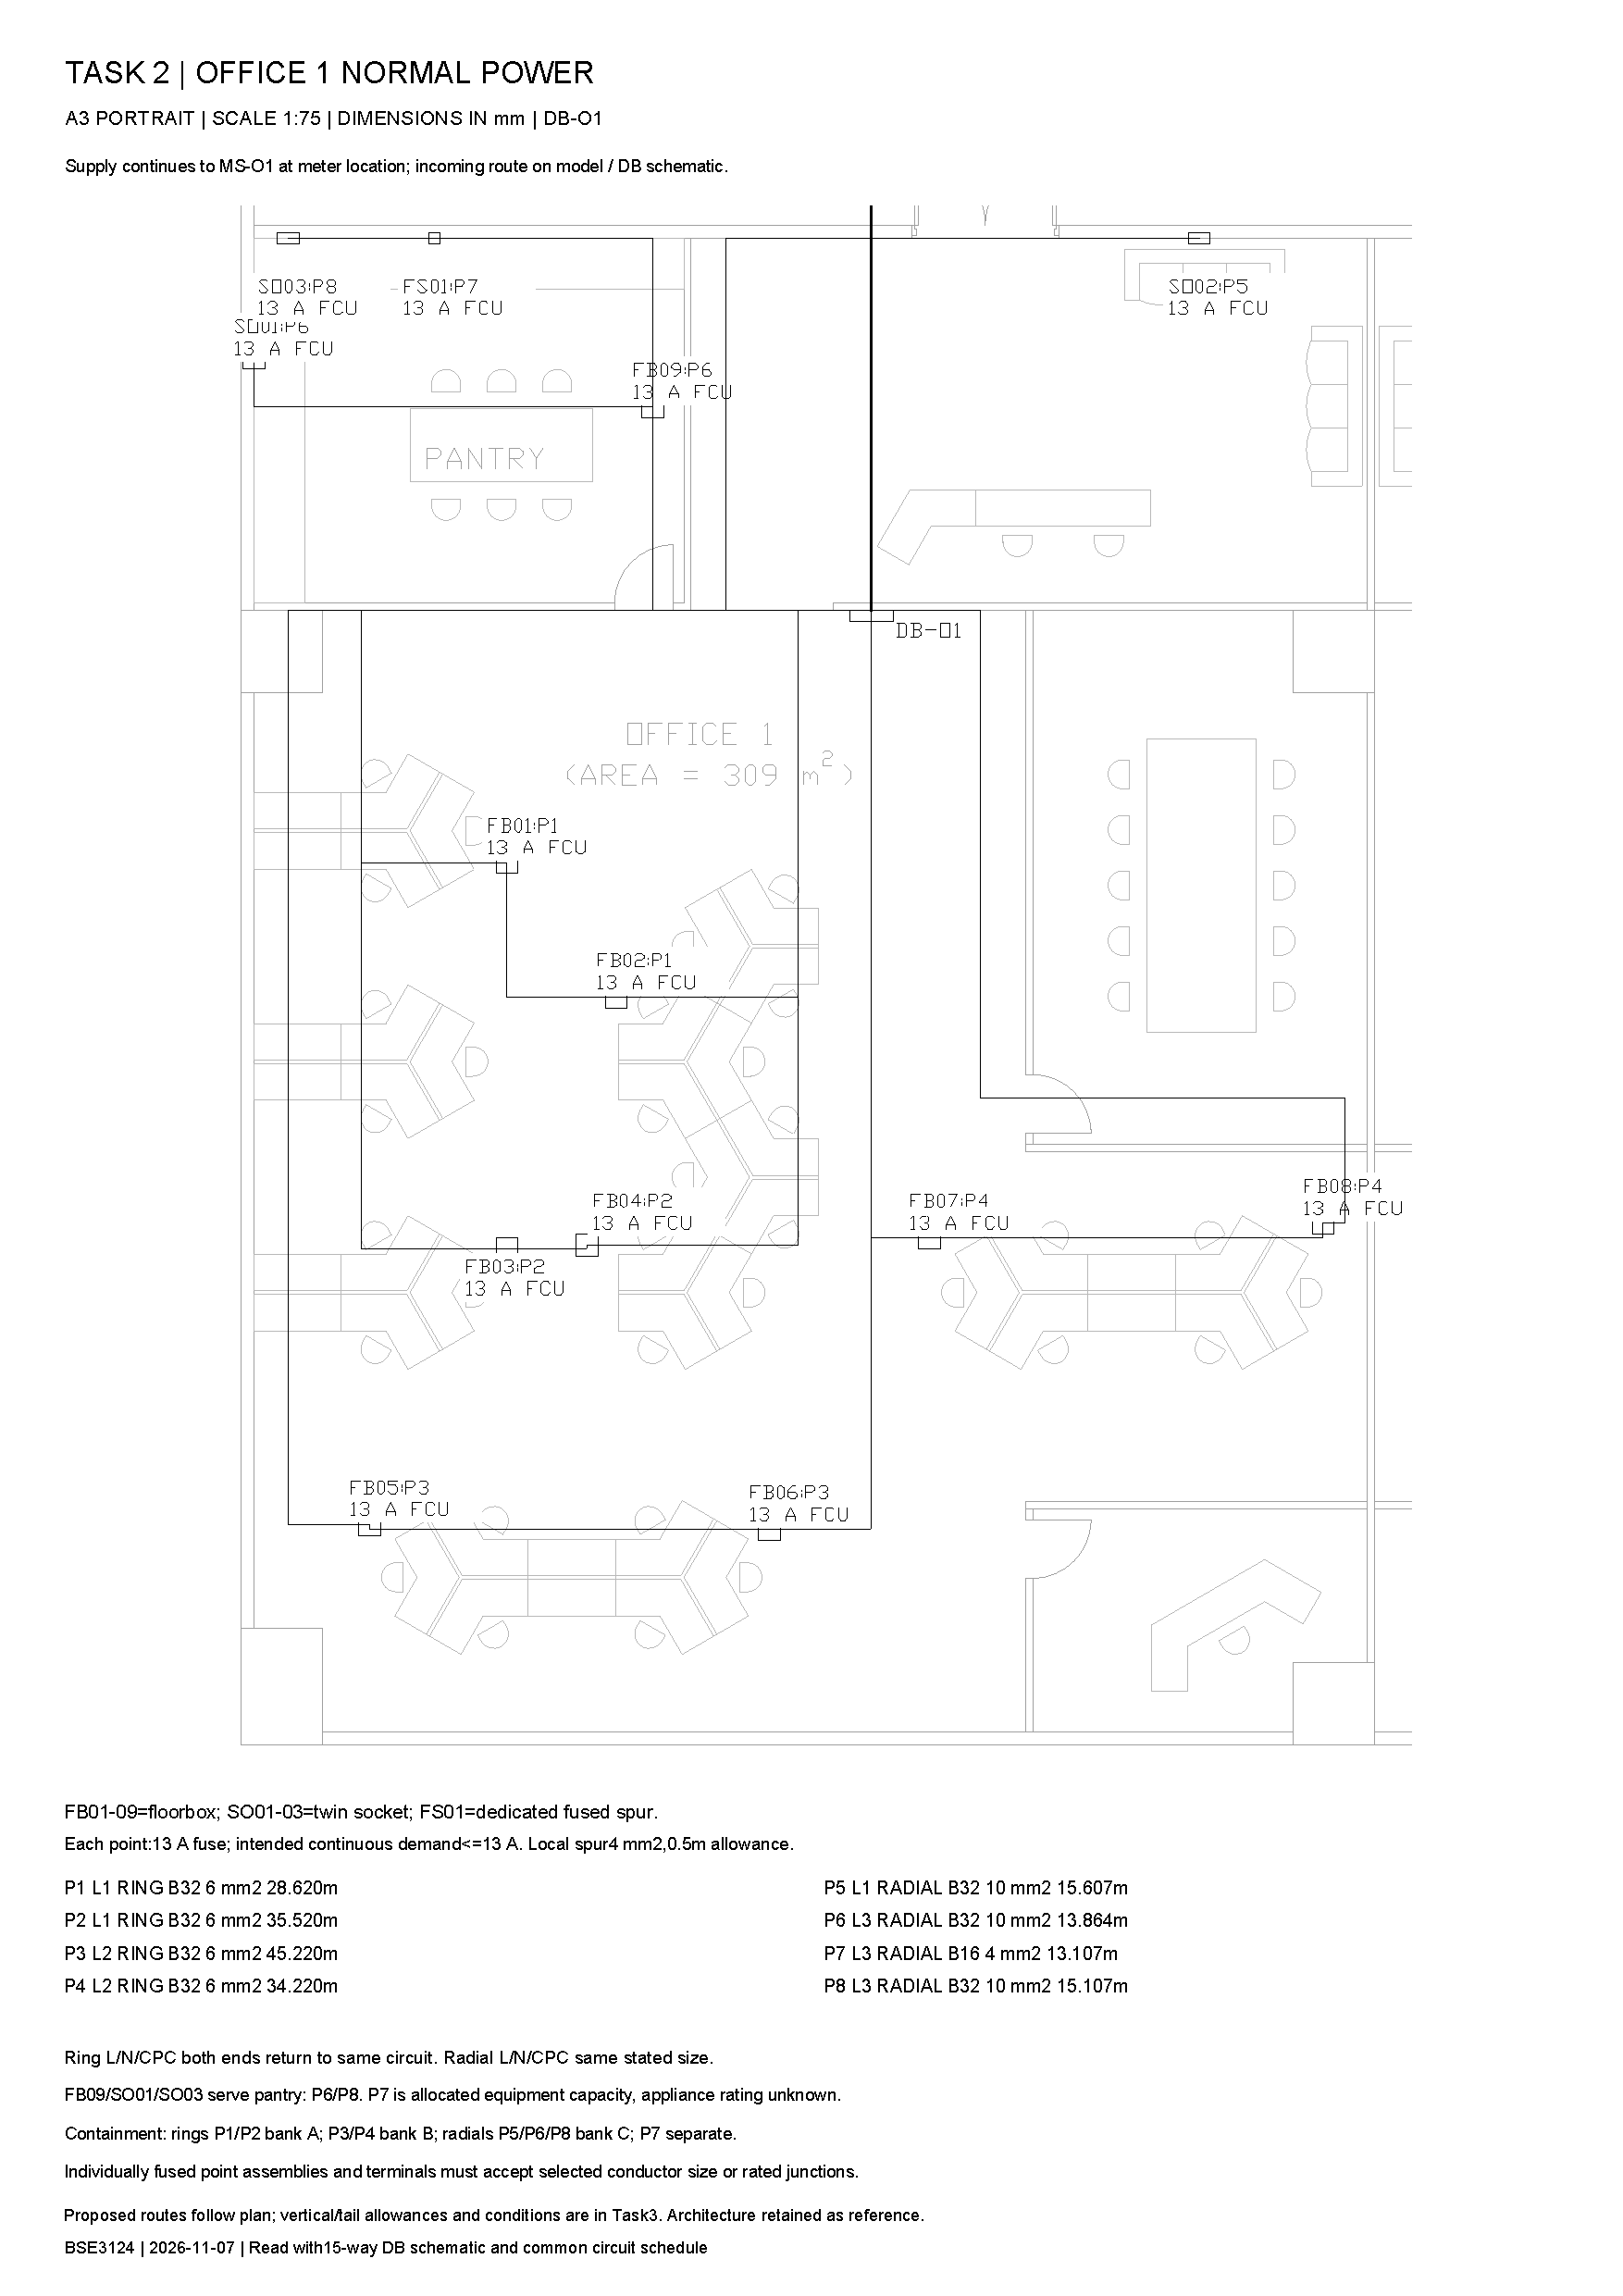
\includepdf[pages=-,fitpaper=true]{assets/office-power.pdf}
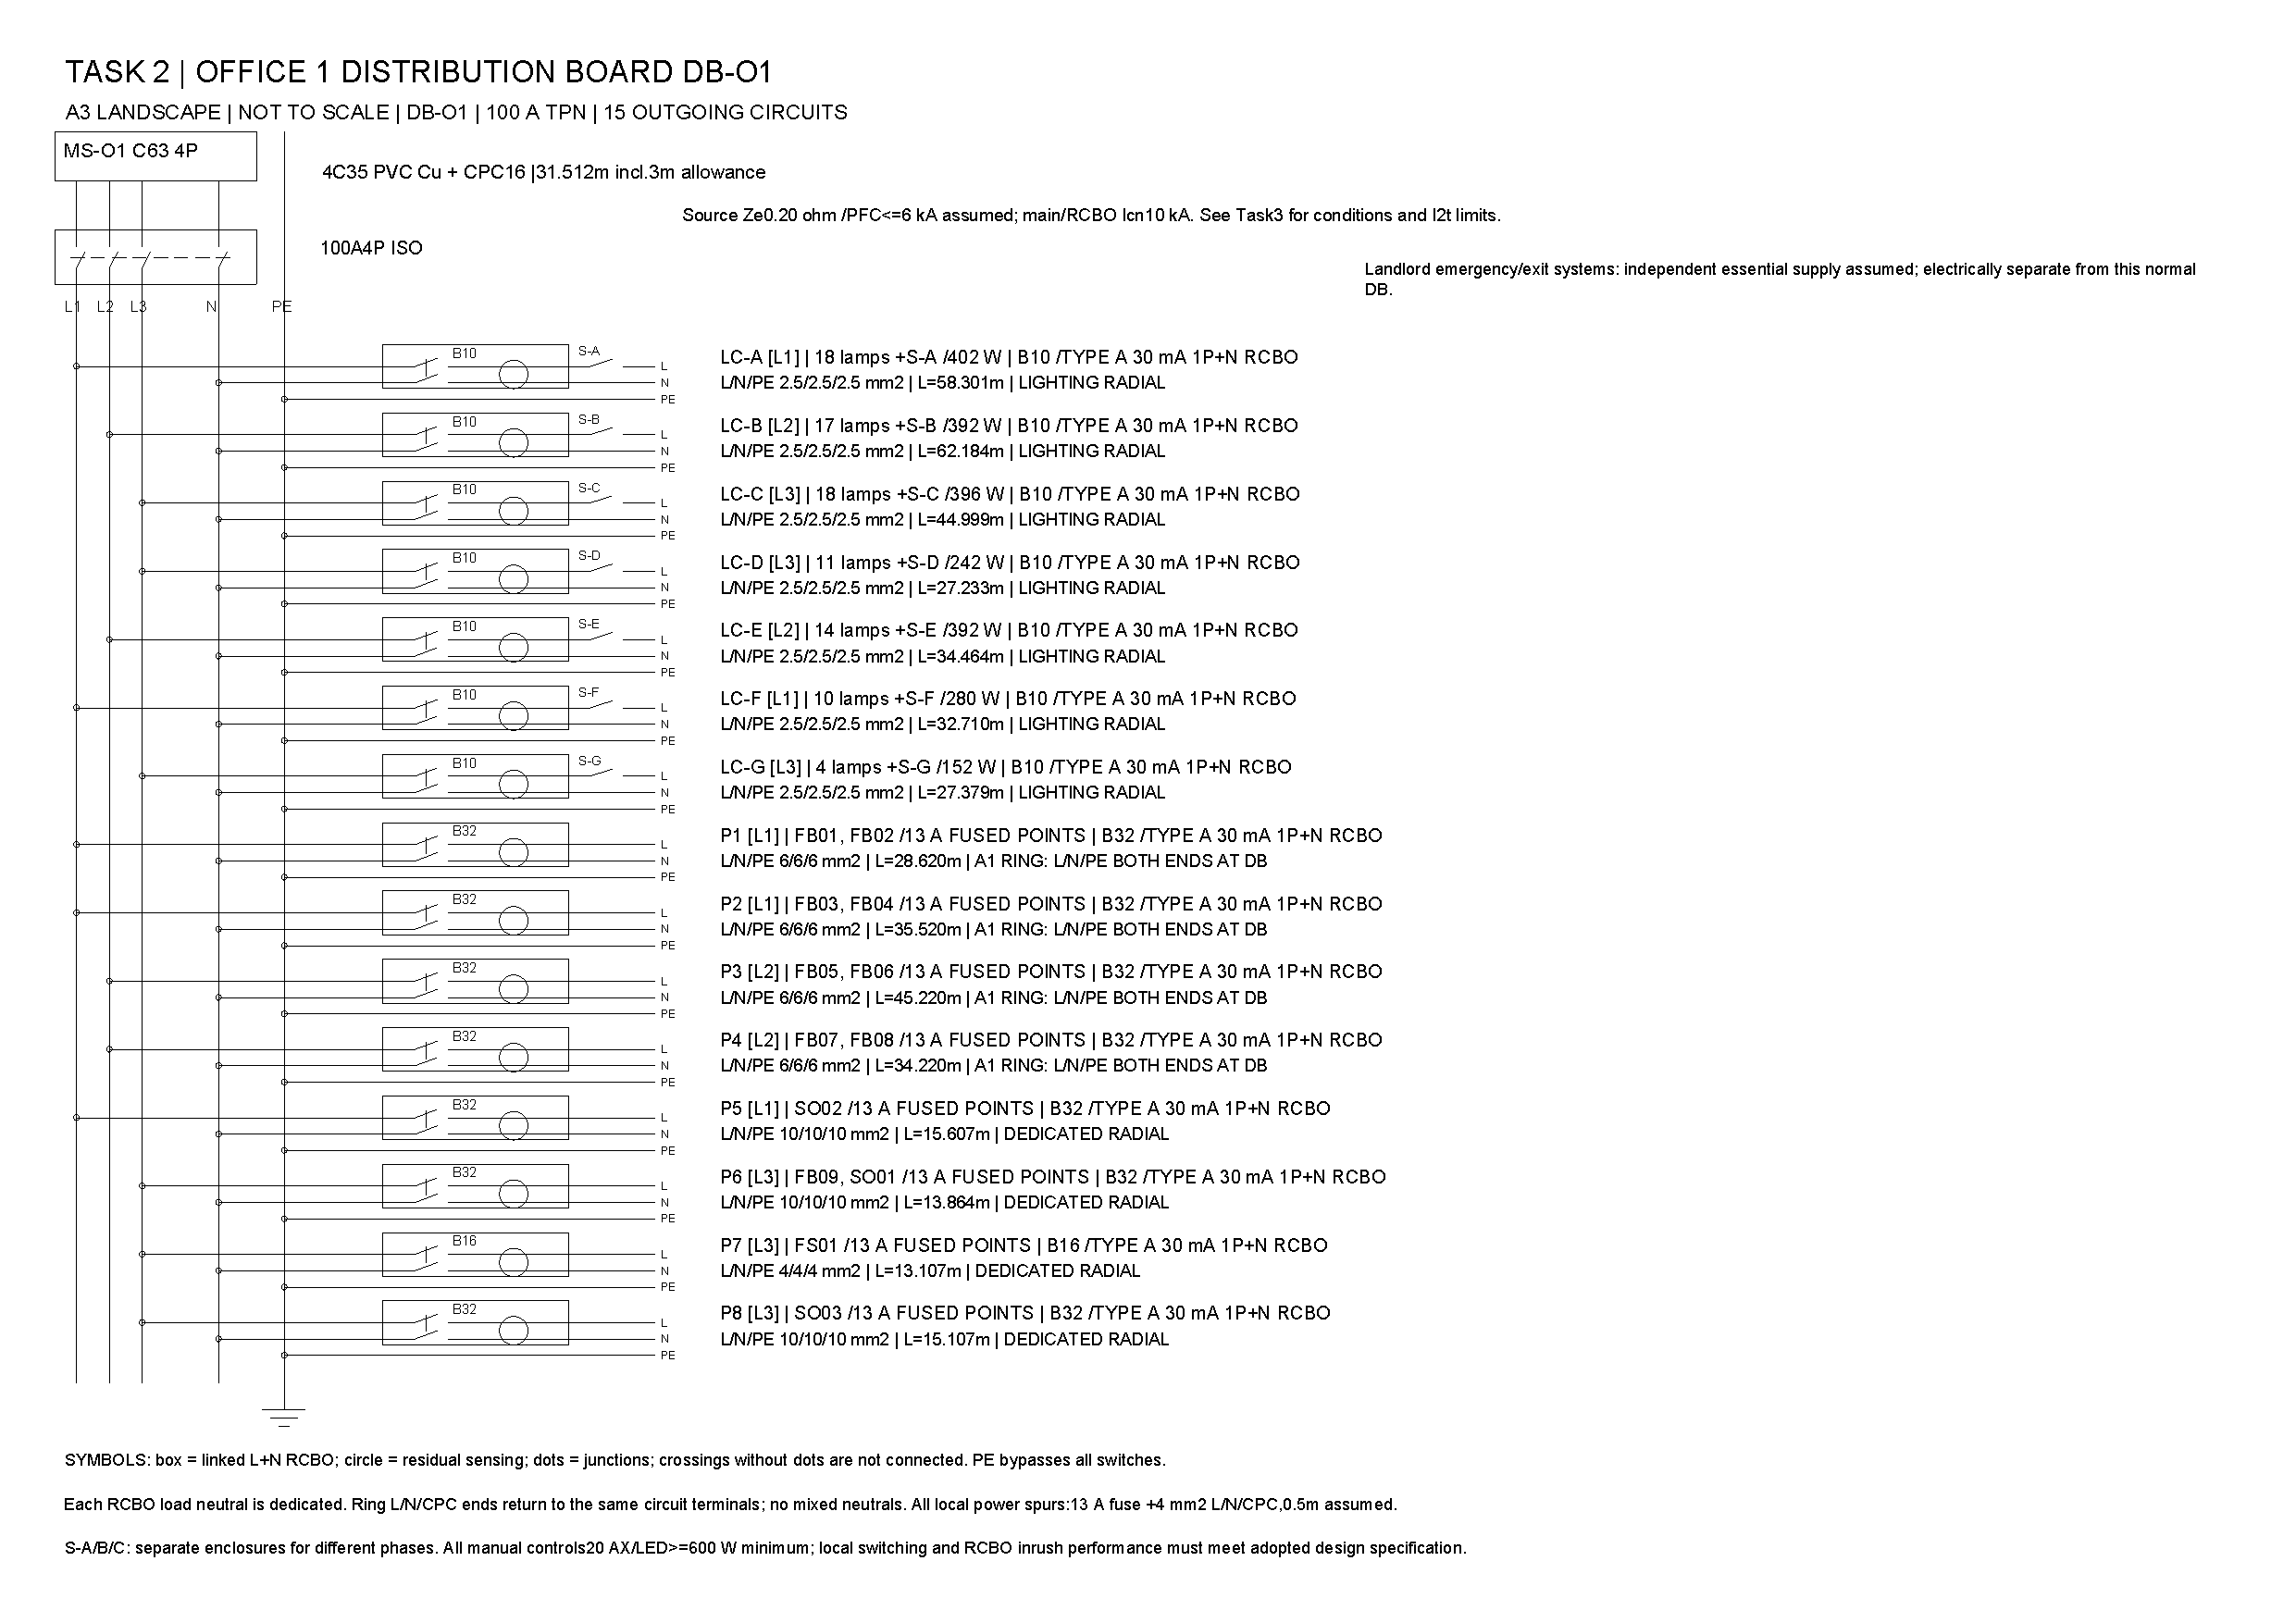
\includepdf[pages=-,fitpaper=true]{assets/office-db.pdf}
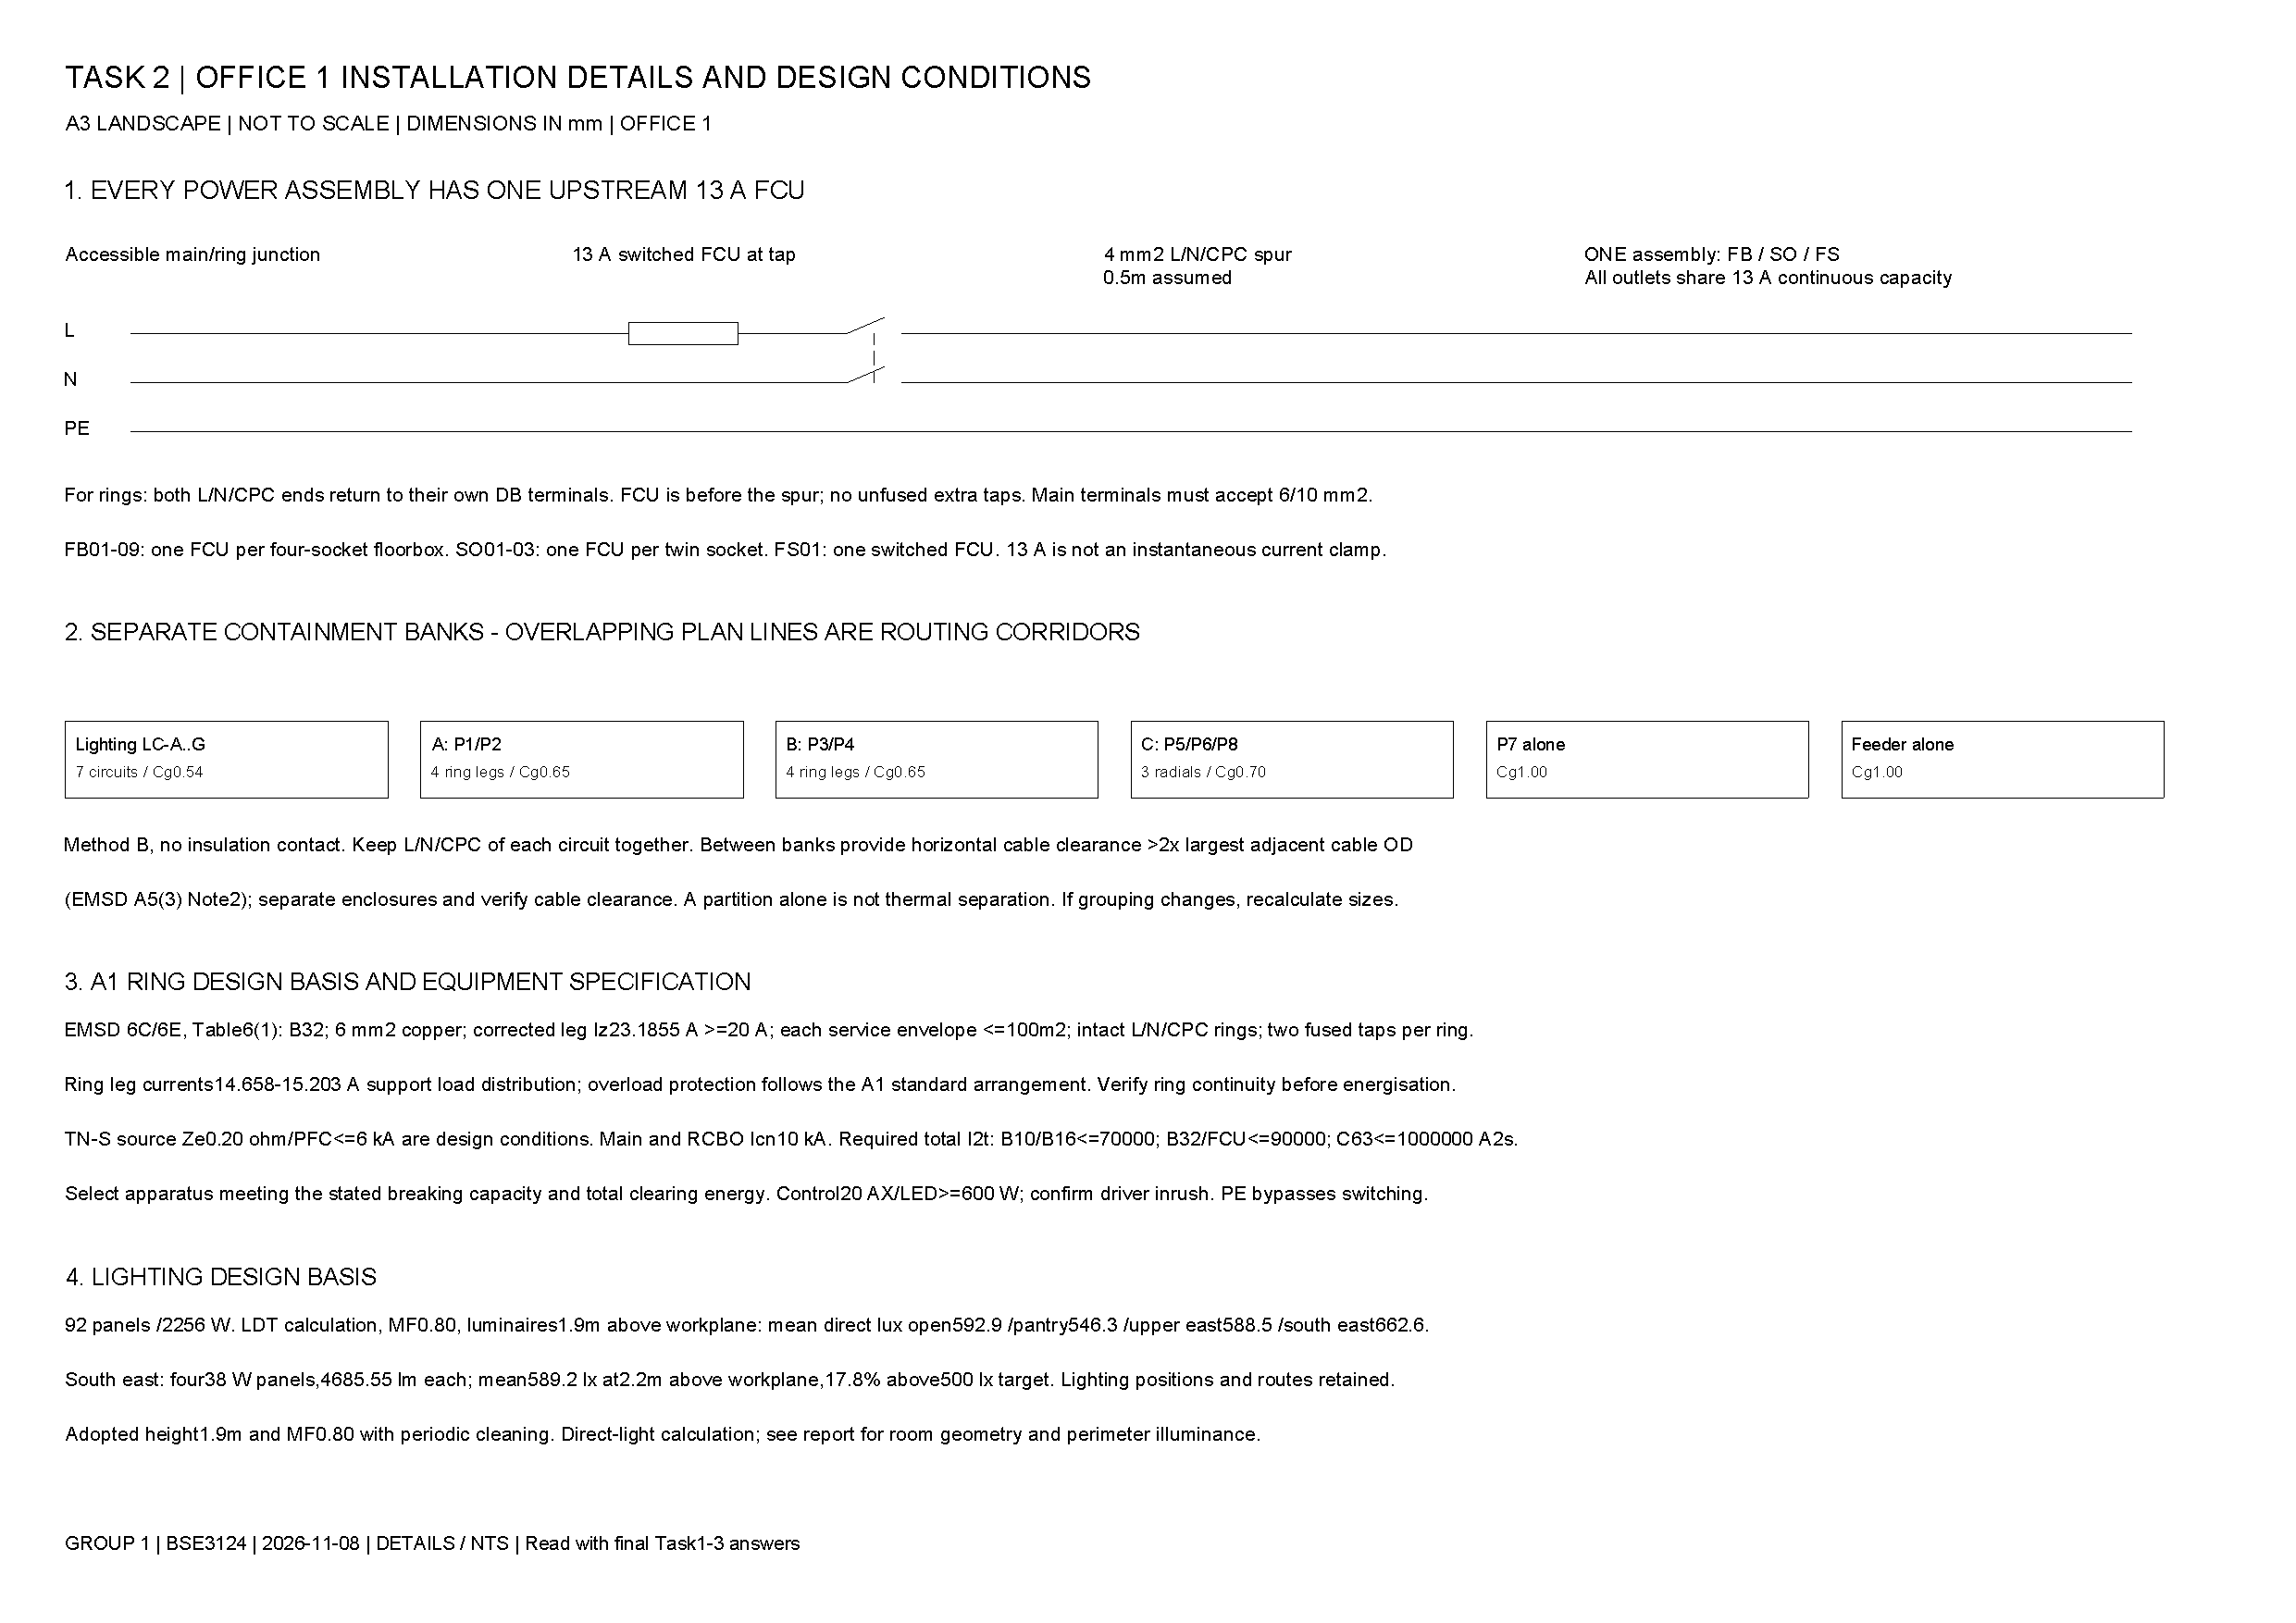
\includepdf[pages=-,fitpaper=true]{assets/installation-details.pdf}
\sheet{4}{\slot{80}{139}{435}{
Lighting current is calculated as $I=P/(220\times0.90)$. Under EMSD Table 7(1), the demand includes 90\% of lighting and 100\% of the largest Code 6E circuit plus 50\% of the remaining circuits on each phase. P7 is allocated separately at 100\%. The 13\,A per assembly is an intended maximum continuous load, not an instantaneous fuse clamp.
\begin{center}\begin{tabular}{lrrrr}\toprule
Phase & Light A$^*$ & Sockets A & Fixed A & Demand A\\\midrule
L1 & 3.444 & 45.500 & 0 & 48.600\\
L2 & 3.960 & 39.000 & 0 & 42.564\\
L3 & 3.990 & 32.500 & 13 & 49.091\\\bottomrule
\end{tabular}\end{center}
$^*$Lighting column is before the 90\% factor. Thus, the maximum demand of \textbf{49.091\,A} leads to the selection of 63\,A source protection and a 100\,A DB. Maximum undiversified phase allowance is 68.444\,A. Full branch currents are retained for outgoing cable sizing.
}
\slot{80}{402}{435}{
The selected feeder is 4-core 35\,mm$^2$ PVC copper plus 16\,mm$^2$ CPC, using Method B. Its 28.5119\,m route plus an assumed 3\,m vertical/termination allowance totals 31.5119\,m. At 40\,$^\circ$C, $C_a=0.87$, $C_g=1$; the calculation adopts $C_h=0.86$ for the stated third-harmonic range (15--33\%).
\begin{align*}
I_{z,25}&=80(0.87)(0.86)=59.856<63\ {\rm A},\\
I_{z,35}&=99(0.87)(0.86)=74.0718\ {\rm A},\\
I_b&=49.091\le I_n=63\le I_z=74.0718\ {\rm A}.
\end{align*}
These ratings follow EMSD A6(2), column 5, while CPC sizing follows Table 11(2)(a). A full-size neutral is retained; neutral current must remain within the adopted bound.

At 63\,A, feeder drop is 2.521606\,V. Including the 2.2\,V pre-origin allowance and calculated branch drops gives a worst complete drop of 3.031\% of 220\,V, below 4\%. The checks assume TN-S, source $Z_e=0.20\,\Omega$ and PFC $\le6$\,kA. Thus, the DB external loop is 0.264129\,$\Omega$; source C63 disconnection and outgoing B-curve checks pass under those conditions.

\textbf{Outgoing circuits are also included}, as required by the assignment: all 15 sizes, currents, lengths, voltage drops, earth-fault checks and apparatus energy requirements are tabulated in the continuation.
}}
\AddToShipoutPictureBG{\AtPageLowerLeft{\includegraphics[page=3,width=\paperwidth,height=\paperheight]{assets/continuation-template.pdf}}}
% !TeX root = main.tex
\subsection*{Incoming design conditions}
The preceding sheet selects C63 protection and a 4-core 35 mm$^2$ feeder with 16 mm$^2$ CPC. Along the meter-to-DB route, the length is 28.5119 m plus a 3 m vertical/termination allowance. Cable sizing assumes 40\,$^\circ$C, a separate Method B enclosure and third-harmonic content greater than 15\% and at most 33\%, giving $C_a=0.87$, $C_g=1$ and $C_h=0.86$. A full-size neutral is retained on this basis.

To bound the phase-neutral voltage drop, the calculation uses $(2/\sqrt3)(1.10)=1.270170592$ mV/A/m from the three-phase table impedance, with neutral current at most 63 A. Thus, feeder drop is 2.521606 V at 63 A and 1.964888 V at the design demand of 49.091 A. Additionally, the complete-path calculation below includes the 2.2 V upstream allowance.

\subsection*{All outgoing cables}
All outgoing cable sizes refer to PVC copper L/N/CPC conductors. Lighting grouped separately has $I_z=24(0.87)(0.54)=11.2752$ A for seven 2.5 mm$^2$ circuits;  all $I_b\le 10\le I_z$. Lighting lengths include 5 m DB/switch vertical allowance.

Each uniform ring bank counts as four current-carrying legs, giving $I_z=41(0.87)(0.65)=23.1855$ A per 6 mm$^2$ leg, above the standard 20 A minimum. With 13 A per point, the ring-network solution gives maximum leg currents 14.658--15.203 A, below $I_z$. However, the radial criterion $I_n\le I_z$ must not be applied to just one ring leg. Continuity and fused-point restrictions are essential.

Meanwhile, the 10 mm$^2$ A2 radial cables have $I_z=57(0.87)(0.70)=34.713$ A;  P7's separate 4 mm$^2$ radial has $I_z=32(0.87)=27.84$ A. In determining route lengths, the power radials include a 2 m vertical allowance, while the rings include 2 m at each DB end. Additionally, each local point spur adds 0.5 m of 4 mm$^2$ cable.
\begin{longtable}{llrrrr}\toprule
Circuit & Phase & $I_b$ A & RCBO A & L/N/CPC mm$^2$ & Main length m\\\midrule\endhead

LC-A & L1 & 2.030 & 10 & 2.5 & 58.301 \\
LC-B & L2 & 1.980 & 10 & 2.5 & 62.184 \\
LC-C & L3 & 2.000 & 10 & 2.5 & 44.999 \\
LC-D & L3 & 1.222 & 10 & 2.5 & 27.233 \\
LC-E & L2 & 1.980 & 10 & 2.5 & 34.464 \\
LC-F & L1 & 1.414 & 10 & 2.5 & 32.710 \\
LC-G & L3 & 0.768 & 10 & 2.5 & 27.379 \\
P1 & L1 & 26.000 & 32 & 6 & 28.620 \\
P2 & L1 & 26.000 & 32 & 6 & 35.520 \\
P3 & L2 & 26.000 & 32 & 6 & 45.220 \\
P4 & L2 & 26.000 & 32 & 6 & 34.220 \\
P5 & L1 & 13.000 & 32 & 10 & 15.607 \\
P6 & L3 & 26.000 & 32 & 10 & 13.864 \\
P7 & L3 & 13.000 & 16 & 4 & 13.107 \\
P8 & L3 & 13.000 & 32 & 10 & 15.107 \\

\bottomrule\end{longtable}
\subsection*{Complete voltage drop and fault checks}
The voltage-drop calculation sums the segment drops using downstream currents on the radials and solves the two-feed ring network, including the stated vertical/local allowances. Combining this result with the 2.2 V pre-origin allowance and the 2.521606 V feeder bound gives the full-path drop, which is checked against a limit of $0.04(220)=8.8$ V.

Fault-protection checks assume a TN-S supply, an external source loop impedance of 0.20 ohm and PFC at most 6 kA at MS-O1/downstream.  Adding the incoming phase+CPC bound of 0.064129 ohm gives a DB external loop impedance of 0.264129 ohm. Table 11(10) reference limits are B10=4.17, B16=2.61, B32=1.31 and C63=0.33 ohm. Throughout these checks, the calculation uses operating-temperature paths and a minimum voltage factor of 0.95. Within a uniform ring, the worst parallel path is at most a quarter of the circumference.
\begin{longtable}{lrrrrr}\toprule
Circuit & Out drop V & Total drop \% & $Z_s$ ohm & Min fault A & $Z_s$ limit ohm\\\midrule\endhead

LC-A & 1.450 & 2.805 & 1.314 & 159.1 & 4.17 \\
LC-B & 1.237 & 2.709 & 1.383 & 151.1 & 4.17 \\
LC-C & 0.959 & 2.582 & 1.074 & 194.6 & 4.17 \\
LC-D & 0.422 & 2.338 & 0.754 & 277.1 & 4.17 \\
LC-E & 0.797 & 2.509 & 0.884 & 236.3 & 4.17 \\
LC-F & 0.642 & 2.438 & 0.853 & 245.0 & 4.17 \\
LC-G & 0.345 & 2.303 & 0.757 & 276.1 & 4.17 \\
P1 & 1.269 & 2.723 & 0.322 & 649.3 & 1.31 \\
P2 & 1.675 & 2.907 & 0.334 & 624.9 & 1.31 \\
P3 & 1.937 & 3.027 & 0.352 & 593.5 & 1.31 \\
P4 & 1.428 & 2.795 & 0.332 & 629.4 & 1.31 \\
P5 & 0.964 & 2.584 & 0.338 & 617.8 & 1.31 \\
P6 & 1.310 & 2.742 & 0.331 & 632.1 & 1.31 \\
P7 & 1.946 & 3.031 & 0.414 & 505.1 & 2.61 \\
P8 & 0.936 & 2.571 & 0.336 & 621.8 & 1.31 \\

\bottomrule\end{longtable}
Under the adopted conditions, all 15 full voltage bounds pass, with a worst-case drop of 3.031\%. Additionally, the calculated minimum earth-fault current in each B-curve final circuit exceeds the threshold $5I_n$. Similarly, incoming C63 gives $Z_s=0.264129<0.33$ ohm and $I_{f,\min}=791.28>10(63)=630$ A, satisfying reference instantaneous disconnection under the adopted conditions.
\newpage
\subsection*{Overload and total clearing energy}
CPC thermal withstand is checked using $k=115$ for bunched PVC copper CPCs initially at 70\,$^\circ$C (11(2)(c)), with total $I^2t\le(kS)^2$ required. Additionally, the main protection and RCBOs must have a breaking capacity of 10 kA. B-curve devices must limit class 3-equivalent total energy to at most 70,000 A$^2$s for B10/B16 and 90,000 for B32. Accordingly, the selected RCBOs must have manufacturer total-clearing-energy data that meet these limits. Corresponding CPC withstands are 82,656.25 (2.5 mm$^2$), 211,600 (4), 476,100 (6) and 1,322,500 (10), each above the required device bound.

Incoming C63 total energy must be at most 1,000,000 A$^2$s over the relevant fault range, below CPC16 withstand 3,385,600. Similarly, complete 13 A FCU energy must be at most 90,000, below the 4 mm$^2$ spur withstand 211,600. Therefore, the incoming breaker and FCU assemblies must be selected to meet these total-energy limits.

Under fuse overload conditions, $I_2=1.9(13)=24.7$ A. Spur $I_z=32(0.87)(0.70)=19.488$ A gives $1.45I_z=28.2576>24.7$ A. Overload suitability of P1--P4 is assessed using the standard A1 arrangement in EMSD 6C, 6E and Table 6(1), Note 1(i): 32 A protection, copper size at least 2.5 mm$^2$, corrected per-leg capacity at least 20 A, served area at most 100 m$^2$, intact L/N/CPC rings and evenly distributed outlets. On this basis, the adopted 6 mm$^2$ rings meet these conditions. Exactly two individually 13 A fused connections are allowed per ring; no additional unfused taps are permitted. Here, the leg-current calculation checks load distribution; the A1 standard arrangement governs ring overload protection. With a reference interruption rating of 6 kA, the fuse meets the assumed PFC of at most 6 kA. However, its typical pre-arcing 870 A$^2$s is \emph{not} total clearing energy. Finally, the design assumes an FCU ambient temperature of at most 35\,$^\circ$C and a board apparatus ambient temperature of at most 30\,$^\circ$C; a containment temperature of 40\,$^\circ$C remains the conservative cable condition.
\subsection*{References}
CLP COP215 Rev 07: clauses 3.1.7 and 3.3.1; Appendices 2 and 7 (building demand). CLP COP101 v16: clauses 4.3, 5.5, 5.6 and 6.1--6.7 (plantroom planning).

EMSD Code of Practice for the Electricity (Wiring) Regulations, 2025: Table 6(1), printed p.56; Table 7(1), pp.65--67; 9B, p.79; Table 11(2), pp.99--100; Table 11(10), p.105; Appendix 5 correction factors and Appendix 6 cable ratings.

Performance in Lighting, PLATO 600 MultiPower 3117955: LOW (22 W), MEDIUMLOW (28 W) and HIGH (38 W) manufacturer LDT files, October 2022. ABB guide 9AKK108468A3912, p.130: B-curve energy references. Eaton TDC180 Technical Data 2042, August 2024, p.2: fuse conventional-fusing and interruption data. Total FCU clearing energy is specified separately above.

\noindent Electrical Schematic 1: transformer, main LV switchboard and floor-metering arrangement. Electrical Schematic 2: final distribution-board schematic conventions.

\clearpage\ClearShipoutPictureBG
\end{document}
